%%%%%%%%%%%%%%%%%%%%%%%%%%%%%%%%%%%%%%%%%
% baposter Landscape Poster
% LaTeX Template
% Version 1.0 (11/06/13)
%
% baposter Class Created by:
% Brian Amberg (baposter@brian-amberg.de)
%
% License:
% CC BY-NC-SA 3.0 (http://creativecommons.org/licenses/by-nc-sa/3.0/)
%
%%%%%%%%%%%%%%%%%%%%%%%%%%%%%%%%%%%%%%%%%

%----------------------------------------------------------------------------------------
% PACKAGES AND OTHER DOCUMENT CONFIGURATIONS
%----------------------------------------------------------------------------------------

\documentclass[landscape,a0paper,fontscale=0.285]{baposter} % Adjust font scale/size

\usepackage{graphicx} % Required for including images
\graphicspath{{figs/}} % Directory in which figures are stored

\usepackage{amsmath} % For typesetting math
\usepackage{amssymb} % Adds new symbols to be used in math mode
\usepackage{mathtools}

\usepackage[numbers]{natbib}

\usepackage{booktabs} % Top and bottom rules for tables
\usepackage{enumitem} % Used to reduce itemize/enumerate spacing
\usepackage{palatino} % Use the Palatino font
\usepackage[font=small,labelfont=bf]{caption} % Required for specifying captions to tables and figures

\usepackage{multicol} % Required for multiple columns
\setlength{\columnsep}{1.5em} % Slightly increase the space between columns
\setlength{\columnseprule}{0mm} % No horizontal rule between columns

\newcommand{\compresslist}{ % Define a command to reduce spacing within itemize enumerate environments, this is used right after \begin{itemize} or \begin{enumerate}
\setlength{\itemsep}{1pt}
\setlength{\parskip}{0pt}
\setlength{\parsep}{0pt}
}

\definecolor{lightblue}{rgb}{0.145,0.6666,1} % Defines color of content box headers

\begin{document}

\begin{poster} {
headerborder=closed, % Adds a border around the header of content boxes
colspacing=1em, % Column spacing
bgColorOne=white, % Background color for the gradient on the left side of the poster
bgColorTwo=white, % Background color for the gradient on the right side of the poster
borderColor=lightblue, % Border color
headerColorOne=black, % Background color for the header in the content boxes (left side)
headerColorTwo=lightblue, % Background color for the header in the content boxes (right side)
headerFontColor=white, % Text color for the header text in the content boxes
boxColorOne=white, % Background color of the content boxes
textborder=roundedleft, % Format of the border around content boxes, can be: none, bars, coils, triangles, rectangle, rounded, roundedsmall, roundedright or faded
eyecatcher=true, % Set to false for ignoring the left logo in the title and move the title left
headerheight=0.1\textheight, % Height of the header
headershape=roundedright, % Specify the rounded corner in the content box headers, can be: rectangle, small-rounded, roundedright, roundedleft or rounded
headerfont=\Large\bf\textsc, % Large, bold and sans serif font in the headers of content boxes
%textfont={\setlength{\parindent}{1.5em}}, % Uncomment for paragraph indentation
linewidth=2pt % Width of the border lines around content boxes
}
%----------------------------------------------------------------------------------------
% TITLE SECTION
%----------------------------------------------------------------------------------------
%
{
\includegraphics[height=6.5em]{logo_berkeley.jpg}} % First university/lab logo on the left
{\bf\textit{\LARGE Robust Nonparametric Inference for Stochastic Interventions
    Under Multi-Stage Sampling}\vspace{0.01em}} % Poster title
{\textbf{Nima S.~Hejazi, Mark J.~van der Laan, and David C.~Benkeser} \\
  \textit{Group in Biostatistics \& Department of Statistics, University of
    California, Berkeley} \\
  \textit{Department of Biostatistics and Bioinformatics, Emory University}}
    % Author names and institution
{
\includegraphics[height=6.5em]{logo_emory.jpg}} % Second university/lab logo on the right

%-------------------------------------------------------------------------------
% OVERVIEW
%-------------------------------------------------------------------------------

\headerbox{Overview \& Motivations}{name=overview,column=0,row=0}{

\begin{enumerate}\compresslist
\setlength\itemsep{0.5em}
\item We consider the problem of efficiently estimating the effect of a
 stochastic shift interventions for problem settings in which multi-stage
 sampling complicates the observed data structure.
\item We present a novel approach: an augmented targeted maximum likelihood
 estimator of a parameter defined as the outcome under a stochastic
 intervention with
  \begin{itemize}
    \item consistency and efficiency guarantees even under multi-stage
      sampling, and
    \item a form of multiple double robustness inherited from its constituent
      parts.
  \end{itemize}
\item The proposed nonparametric estimation procedure provably attains fast
  convergence rates even when incorporating machine learning estimators.
\item A recent software implementation --- the ``\textit{txshift}'' R package
  \cite{hejazi2018txshift} --- has been developed for applying this methodology
  in complete generality, including for causal inference and variable importance
  analyses.
\end{enumerate}

%\vspace{0.3em} % When there are two boxes, some whitespace may need to be added
               % if the one on the right has more content
}

%-------------------------------------------------------------------------------
% INTRODUCTION
%-------------------------------------------------------------------------------

\headerbox{Data: HIV Vaccine Trials}
{name=introduction,column=1,row=0,bottomaligned=overview}{

\begin{itemize}\compresslist
\setlength\itemsep{0.5em}
\item We illustrate the utility of our approach by applying the new method and
  software in an investigation of the effects of immune response biomarkers on
  HIV vaccine efficacy.
\item \textit{Question of interest:} \textbf{How does risk of HIV infection
   differ under posited shifts of the distribution of an immune response in the
   vaccine arm of an efficacy trial?}
\item We simulate a data structure based on the HVTN 505 HIV-1 efficacy trial,
  as in \cite{janes2017higher}:
  \begin{itemize}
    \itemsep0.5pt
    \item About 2500 participants, with all observed cases matched to controls.
    \item Background $(W)$: sex, age, BMI, etc.
    \item Intervention $(A)$: immunobiomarkers (i.e., T-Cell profiles from ICS
      assays on preserved HIV-1-stimulated PBMCs).
    \item Outcome $(Y)$: HIV-1 infection status.
  \end{itemize}
\item \textit{Takeaway:} \textbf{Variable importance measure for ranking
   multiple immune responses by their utility as immunogenicity study endpoints
   in future HIV-1 vaccine trials.}
\end{itemize}
}

%-------------------------------------------------------------------------------
% Methodology cont.
%-------------------------------------------------------------------------------

\headerbox{Methodology II: Corrections for Multi-Stage Sampling}{name=results,
  column=2,span=2,row=0}{

\vspace{-0.35em}
\begin{itemize}
\item In the HVTN 505 HIV-1 trial, all infected individuals are matched to
  controls using a complex mechanism, which makes the observed data structure
  \textbf{$O = (W, \Delta A, Y)$}, where
  \begin{itemize}
    \itemsep0.25pt
    \item $V = (W, Y)$ is the set of variables defining the sampling mechanism,
    \item $\Delta = f(V) \in \{0, 1\}$ is the missingness mechanism introduced
      by sampling,
    \item $\Pi_0(V) = \mathbb{P}(\Delta = 1 \mid V)$, letting $\Pi_n(V)$ be an
      estimator of $\Pi_0(V)$.
  \end{itemize}
\item An IPCW-TMLE, introduced by \cite{rose2011targeted2sd}, augments the loss
  function with IPC weights to overcome the problem introduced by sampling:
  $\mathcal{L}(P_X)(O) = \frac{\Delta}{\Pi_n(V)}\mathcal{L}^F(P_X)(X)$, for full
  data $X = (W, A, Y)$.
\item When working in a nonparametric model, the efficient influence function
  estimating equation is complexified by sampling:
  $0 = P_n \frac{\Delta}{\Pi_n^*(V)}D^F(P^*_{X,n}) -
    \left\{\frac{\Delta}{\Pi_n^*(V)} - 1 \right\} \mathbb{E}_n(D^F(P^0_{X,n})
    \mid \Delta = 1, V)$.
\item Fortuitously, this augmented estimator exhibits a unique form of
  \textit{multiple double robustness} --- through combinations of the terms
  $(g, Q)$ and $(\Pi, \mathbb{E}_0(D^F(P^F) \mid V))$.
\end{itemize}
}

%-------------------------------------------------------------------------------
% REFERENCES
%-------------------------------------------------------------------------------

\headerbox{Principal References}{name=references,column=2,above=bottom}{
\renewcommand{\section}[2]{\vskip 0.05em} % remove "References" section title
\tiny{ % Reduce the font size in this block
\setlength{\bibsep}{0.25pt}
\bibliographystyle{plainnat}
\nocite{*} % Insert publications even if they are not cited in the poster
\bibliography{2018_acic}
\compresslist
\vspace{-0.7em}
}
}

%-------------------------------------------------------------------------------
% CONTACT
%-------------------------------------------------------------------------------

\headerbox{Contact Information}{name=ack,column=3,aligned=references,above=bottom}{
% This block is as tall as the references block
\begin{itemize}
  \itemsep0.25pt
  \item \textbf{N.S.~Hejazi}, Ph.D.~student, Group in Biostatistics,
    \textsc{nhejazi@berkeley.edu}
  \item \textbf{M.J.~van der Laan}, Professor of Biostatistics \& Statistics,
    \textsc{laan@berkeley.edu}
  \item \textbf{D.C.~Benkeser}: Assistant Professor of Biostatistics,
    \textsc{benkeser@emory.edu}
\end{itemize}
}

%-------------------------------------------------------------------------------
% CONCLUSION
%-------------------------------------------------------------------------------

\headerbox{Results \& Discussion}
{name=conclusion,column=2,span=2,row=0,below=results,above=references}{

\vspace{0.25em}
\begin{multicols}{2}

\begin{center}
\vspace*{-0.5cm}
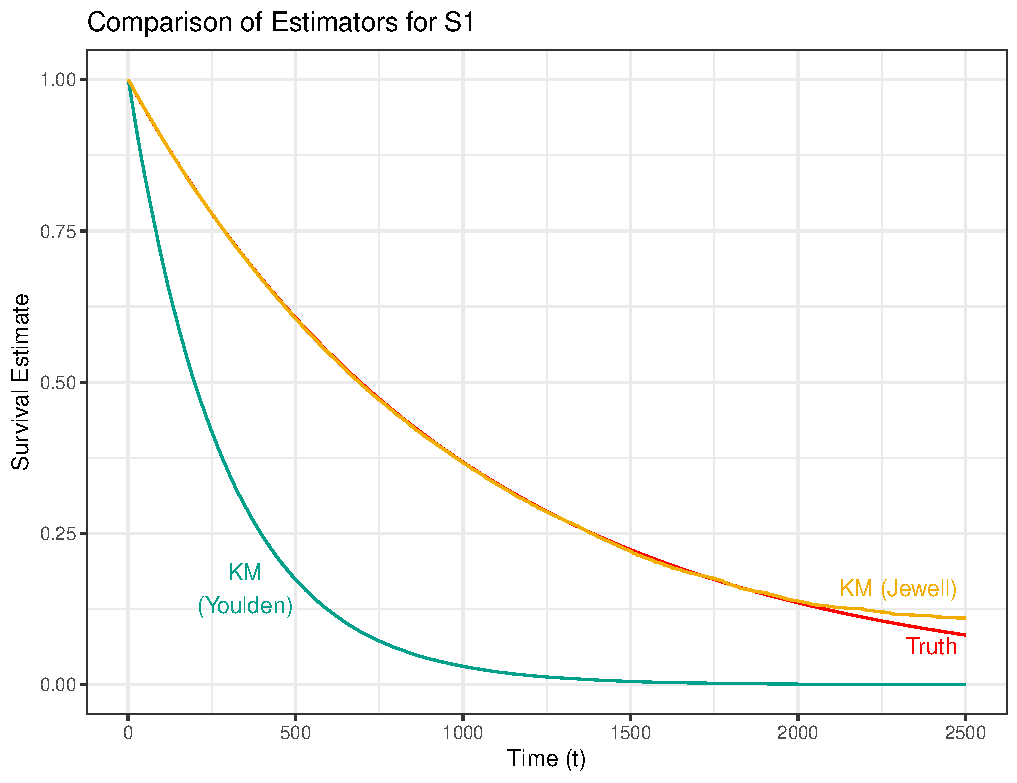
\includegraphics[scale=0.45]{s1_estim_compare}
\vspace{-1.75em}
\captionof{figure}{This figure demonstrates...}
\end{center}

\vspace{-1.75em}

\begin{itemize}
  \itemsep0.05pt
  \item ...
  \item ...
  \item ...
\end{itemize}

\begin{center}
\vspace*{-0.93cm}  % CHANGE THIS TO ALIGN IMAGES
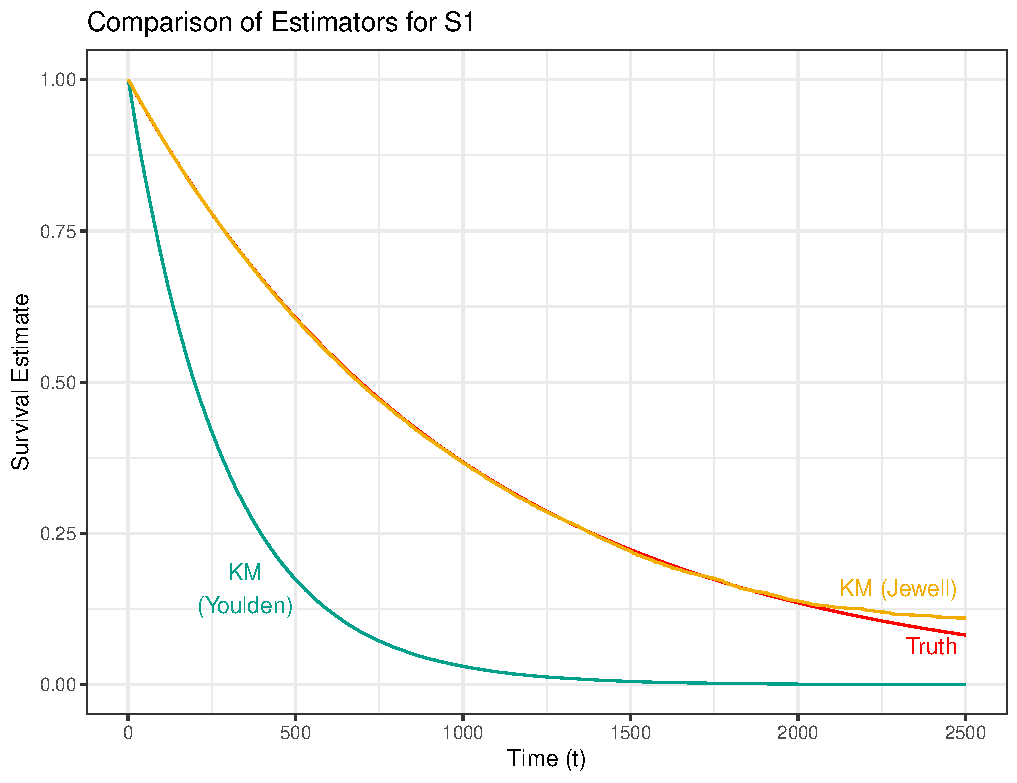
\includegraphics[scale=0.45]{s1_estim_compare}
\vspace{-1.75em}
\captionof{figure}{This figure demonstrates...}
\end{center}

\vspace{-1.75em}

\begin{itemize}
  \itemsep0.05pt
  \item ...
  \item ...
  \item ...
\end{itemize}

\end{multicols}
}

%-------------------------------------------------------------------------------
% METHODS
%-------------------------------------------------------------------------------

\headerbox{Methodology I: The Effect of a Stochastic
  Intervention}{name=method,column=0,span=2,below=overview,
  bottomaligned=references}{
% This block's bottom aligns with the bottom of the conclusion block

\begin{itemize}
  \itemsep1pt
  \item Consider $O = (W, A, Y) \sim P_0 \in \mathcal{M}$, with no assumptions
    placed on the statistical model $\mathcal{M}$.
  \item Rather than a deterministic intervention, consider a shift of the
    treatment (i.e., instead of $A = a$, consider a shift of the intervention so
    that $A = a + \delta$ for an aribtrary $\delta$).
  \item As a comparison with the general linear model, the shift $\delta$ may be
    thought of as a part of the nonparametric analog to the slope of a
    regression line --- i.e., $\beta^{\text{NP}}_{\text{slope}} =
      \frac{\mathbb{E}[Y \mid A + \delta] - \mathbb{E}[Y \mid A]}{\delta^2}$.
  \item To protect against positivity violations, make the shifting mechanism a
    function of the observed data: $d(a, w) = a + \delta$, if
    $a + \delta < u(w)$ and $d(a, w) = a$ otherwise.
\end{itemize}

We consider a simple causal target parameter, introduced in
  \cite{munoz2012population}:
\begin{equation}
\Psi(P) = \mathbb{E}_{\text{P}}{\overline{Q}(d(A, W), W)},
\end{equation}
for which the efficient influence function (EIF), given in
  \cite{diaz2018stochastic}, is
\begin{equation}
D(P)(o) = H(a, w){y - \overline{Q}(a, w)} + \overline{Q}(d(a, w), w) - \Psi(P),
\end{equation}
where the auxiliary term, $H(a,w)$, takes the form
  $H(a,w) = \mathbb{I}(a < u(w)) \frac{g_0(a - \delta \mid w)}{g_0(a \mid w)} +
    \mathbb{I}(a \geq u(w) - \delta)$.\\[0.5em]
We obtain Wald-style inference via the limiting distribution:
$\sqrt{n}(\Psi_n - \Psi) \to N(0, \text{Var}(D(P_0)))$.
}

%-------------------------------------------------------------------------------

\end{poster}
\end{document}

